\section{Serving and API Stability}
\label{sec:gpt54-serving-stability}

Sustaining a single agent for 12 hours or more stresses API serving far more than short evaluations do: a day-long run must keep the model, its context, and its tool calls available without interruption, and any serving-side incident in that window can truncate or degrade the trajectory. Our long-horizon tasks therefore unavoidably fold serving stability into what they measure. We view this as appropriate rather than a confound to be engineered away: an agent deployed to work for hours in the real world is subject to exactly these serving realities, so a benchmark for long-horizon learning should reflect them too.

\begin{center}
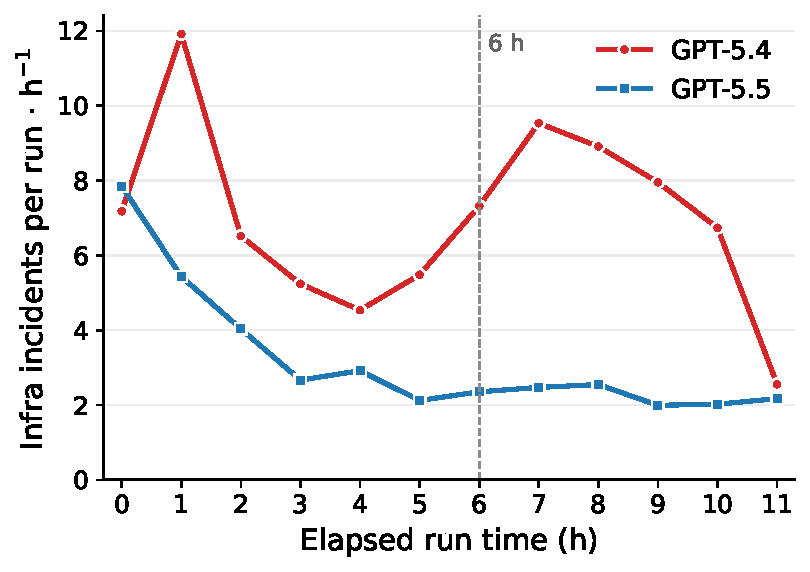
\includegraphics[width=0.52\linewidth]{figures/fig_codex_infra_paper.pdf}
\captionof{figure}{Serving-side incident rate during long-horizon GPT-5.4 and GPT-5.5 runs. Incidents are normalized by active run time; the dashed line marks six elapsed hours. GPT-5.4 experienced substantially more infrastructure and API interruptions, especially in the later part of the run.}
\label{fig:gpt54-serving-stability}
\end{center}

Figure~\ref{fig:gpt54-serving-stability} quantifies this for the two GPT models, plotting the serving-side incident rate (normalized by active run time) against elapsed time: GPT-5.4 saw substantially more infrastructure and API interruptions than GPT-5.5, especially after the six-hour mark. This carries two caveats for GPT-5.4. First, several of the per-task cells with fewer than three valid runs (marked with $\ast$ in the score tables) involve GPT-5.4, so its lower run coverage partly reflects serving reliability rather than model behavior, though the reported scores still use only valid trajectories. Second, it offers an operational explanation for the forecast deviation flagged in Section~\ref{sec:log-sigmoid-fit} (Figure~\ref{fig:sigmoid-forecast-6p5h}): with availability dropping in the second half of the run, GPT-5.4's later trajectory is noisier and pulls away from the log-sigmoid forecast fit to its first 6.5 hours.
